\documentclass[11pt]{article}
    \title{\textbf{Math 217 Homework I}}
    \author{Khac Nguyen Nguyen}
    \date{}
    
    \addtolength{\topmargin}{-3cm}
    \addtolength{\textheight}{3cm}
    
\usepackage{amsmath}
\usepackage{mathtools}
\usepackage{amsthm}
\usepackage{amssymb}
\usepackage{xfrac}
\usepackage{hyperref}
\usepackage{pgfplots, pgfplotstable}
\pgfplotsset{compat=1.8}


\pgfplotstableset{
    create on use/x/.style={
        create col/expr={
            \pgfplotstablerow/201*2-1
        }
    },
    create on use/y/.style={
        create col/expr accum={
            \pgfmathaccuma+(2/201)*(abs(\pgfmathaccuma^2)+abs(\thisrow{x}^2)-1)
        }{0.6}
    }
}


\pgfplotstablenew{201}\loadedtable

\begin{document}
\section*{9 p.33}
\begin{equation*}
    \begin{aligned}
        &y'(t)-y(t) = 2te^{2t} \\
        \implies &y'(t)e^{-t} -y(t)e^{-t} = 2te^t \\
        \implies &\frac{d}{dt} (y(t)e^{-t}) = 2te^t  \\
        \implies & y(t)e^{-t} = 2(t+1)e^{-t} + C \\
        \implies &y(t) = -2(t+1) + Ce^{t} \\
        \implies &y(t) = -2(t+1) + 3e^{t}
    \end{aligned}
\end{equation*}
as $y(0)=1$.
\newpage
\section*{12 p.33}
Let $\mu(t) = e^{\int \frac{t+1}{t}dt} =e^{t+\ln(t)}$
\begin{equation*}
    \begin{aligned}
        &ty'(t) + (t+1)y(t) = t \\
        \implies &y'(t) + \frac{t+1}{t}y(t) = 1 \\
        \implies &\frac{d}{dt}(y(t)\mu(t)) = \mu(t) \\
        \implies &y(t)\mu(t) = \int \mu(t) dt \\
        \implies &y(t) = \int e^{t+\ln(t)} dt \cdot e^{-t-\ln(t)} \\
        \implies &y(t) = (t-1)e^t \cdot e^{-t-\ln(t)} + C \cdot e^{-t-\ln(t)} \\
        \implies &y(t) = (t-1)e^{-\ln(t)} + 4\ln(2) e^{-t-\ln(t)}
    \end{aligned}
\end{equation*}
as $y(\ln(2))=1$.
\newpage
\section*{21 p.34}
\begin{equation*}
    \begin{aligned}
        &y'(t)-\frac{3}{2}y(t) = 3t + 2e^{t} \\
        \implies &y'(t)e^{-\frac{3}{2}t} -\frac{3}{2}y(t)e^{-\frac{3}{2}t} =  (3t + 2e^{t})e^{-\frac{3}{2}t} \\
        \implies &\frac{d}{dt} (y(t)e^{-\frac{3}{2}t}) =  -\dfrac{\mathrm{e}^{-\frac{3t}{2}}\left(12\mathrm{e}^t+6t+4\right)}{3} + C\\
        \implies &y(t) = -\dfrac{12\mathrm{e}^t+6t+4}{3} + Ce^{\frac{3}{2}t} \\
        \implies &y(t) =  -\dfrac{12\mathrm{e}^t+6t+4}{3} +\left(y_0+\frac{16}{3}\right)e^{\frac{3}{2}t} \\
    \end{aligned}
\end{equation*}
as $y(0)=y_0$. Hence, the value of $y_0$ that seperateds solutions that grow positively as $t\to \infty$ and 
negatively is $-\frac{16}{3}$. If $y_0 = \frac{-16}{3}$, then 
\[
    y(t) = - \frac{12e^t + 6t+4}{3}    
\]
Therefore, $y(t) \to - \infty $ as $t \to \infty$.
\newpage
\section*{2 p.40}
\begin{equation*}
    \begin{aligned}
        &y'(t) +y^2(t) \sin(x) = 0 \\
        \implies &-\frac{y'(t)}{y^2(t)} = \sin(x) \\
        \implies &\frac{1}{y} = -\cos(x) + C \\
        \implies &y = -\frac{1}{\cos(x)+C}
    \end{aligned}
\end{equation*}
\newpage
\section*{6 p.40}
\begin{equation*}
    \begin{aligned}
        &\frac{dy}{dx} = \frac{x^2}{1+y} \\
        \implies & (1+y)dy = x^2dx \\
        \implies &y^2+y = \frac{x^3}{3} + C \\
        \implies &y^2+y - \frac{x^3}{3} = C
    \end{aligned}
\end{equation*}
\newpage
\section*{28 p.41}
Let $y = xu$, then 
\begin{equation*}
    \begin{aligned}
        &\frac{dy}{dx} = \frac{4y-3x}{2x-y}  \\
        \implies &u+ x\frac{du}{dx} = \frac{4ux - 3x}{2x-ux} = \frac{4u-3}{2-u} \\
        \implies &x\frac{du}{dx} = \frac{4u-3-2u+u^2}{2-u} \\
        \implies &\frac{2-u}{u^2+2u-3} du= \frac{1}{x} dx \\
        \implies &\int \frac{1/4}{u-1} + \frac{-5/4}{u+3}du = \ln|x| + C \\
        \implies &\frac{1}{4} \ln|u-1| - \frac{5}{4} \ln|u+3| - \ln|x| = C \\
        \implies &\ln \left(|u-1|^{-1/4} |u+3|^{5/4} |x|\right) = C \\
        \implies &|u-1|^{-1/4} |u+3|^{5/4} |x| = e^C > 0 \\
        \implies &|u-1|^{-1} |u+3|^{5} |x|^4 = e^{4C} > 0 \\
        \implies &|u-1|^{-1} |u+3|^{5} |x|^4 = C > 0 (\text{change } C = e^{4C}) \\
        \implies &\left(\frac{y}{x} - 1\right)^{-1} \left( \frac{y}{x} +3 \right)^5 x^4 = C \\
        \implies &(y-x)(y+3x) = C
    \end{aligned}
\end{equation*}
\newpage
\section*{2 p.69}
\begin{tikzpicture}
    \begin{axis}[
        xmin = -1, xmax = 3,
    ymin = -3, ymax = 7]
        \addplot[
            samples = 200,
        smooth,
        thick,
        ] {x * (x-1) * (x-2)};
    \end{axis}
\end{tikzpicture} \\
The equilibrum points are $0,1,2$ as $\frac{dy}{dt} = 0$.

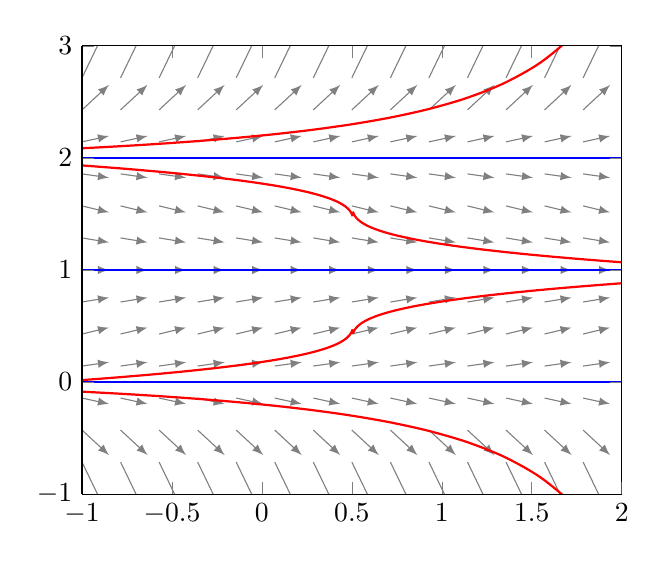
\begin{tikzpicture}
    \begin{axis}[
        view={0}{90},
        domain=-1:2,
        y domain=-1:3,
        xmin=-1, ymin = -1,
        xmax=2, ymax=3,
        samples=15
    ]
    \addplot3 [gray, quiver={u={1}, v={y^3-3*y^2+2*y}, scale arrows=0.15, every arrow/.append style={-latex}}] (x,y,0);
    \addplot [blue, smooth, thick]{2};
    \addplot [blue, smooth, thick]{1};
    \addplot [blue, smooth, thick]{0};
    \addplot [red, smooth, thick]{1/(x-2.5)+0.2};
    \addplot [red, smooth, thick]{-1/(x-2.5) + 1.8};
    \addplot [red, smooth, thick,samples=300]{(0.1*(x-0.5))^(1/3)+0.35};
    \addplot [red, smooth, thick,samples=300]{-(0.1*(-x+0.51))^(1/3)+0.55};
    \addplot [red, smooth, thick,samples=300]{-(0.1*(x-0.5))^(1/3)+1.6};
    \addplot [red, smooth, thick,samples=300]{(0.1*(-x+0.51))^(1/3)+1.4};
    \end{axis}
\end{tikzpicture} \\
We can see that $2,0$ is  unstable and $1$ is asymptotically stable. The red lines are some graphs of solutions, while the blue lines are the phase line.






\end{document}